\documentclass[journal, onecolumn, 12pt]{IEEEtran}
\IEEEoverridecommandlockouts
% The preceding line is only needed to identify funding in the first footnote. If that is unneeded, please comment it out.

\usepackage[justification=centering]{caption}
\usepackage{amsmath,amssymb,amsfonts}
\usepackage{algorithmic}
\usepackage{graphicx}
\usepackage{textcomp}
\usepackage{xcolor}
\usepackage{hyperref}
\usepackage{floatrow}
\newfloatcommand{capbtabbox}{table}[][\FBwidth]

\renewcommand{\baselinestretch}{1.5}

\begin{document}

\title{Lab 5 - Karatsuba polynomial multiplication\\
}

\author{
\IEEEauthorblockN{Şut George-Mihai}
}

\maketitle

\section{Assignment task}
Perform the multiplication of 2 polynomials. Use both the regular $ O(n^2) $ algorithm and the Karatsuba algorithm, and each in both the sequential form and the parallelized form. Compare the 4 variants.

\section{Implementations}
The sequential regular multiplication algorithm is the trivial, normal algorithm for multiplying numbers and polynomials. The parallelized version takes chunks from the polynomials, passes them to threads inside a custom implemented thread pool and multiplies them. (Complexity: $ O(n^2) $)

For the Karatsuba algorithm, we split each polynomial in half recursively and the number of multiplications is reduced by 1. In a classic example of normal multiplication, 4 multiplications are required, while Karatsuba's algorithm only requires 3 multiplications. The parallelized version uses C++ futures with the $ std::async $ function which runs under the $ std::launch::async $ launch strategy to spawn new threads for each of the 3 recursive calls to the Karatsuba function. 
(Complexity: $ O(n^{\log_2 3}) $)

\section{Results}

The most obvious and noticeable detail of the results is that Karatsuba's algorithm only starts to become significantly faster when the polynomial degree is very large. The sequential versions of both the $ O(n^2) $ and $ O(n^{\log_2 3}) $ algorithms have the lowest performance, whereas the parallel versions seem to be the leading methods in terms of execution time. 

Another possible reason why the Karatsuba algorithm seemed to underperform when running tests on polynomials with small degrees is that the variables used for the polynomials inside the function doing the computation are copied in recursive calls, but larger polynomial sizes show a clear advantage of Karatsuba's algorithm over the traditional methods.

Unfortunately, the Karatsuba implementation works only for polynomials of degree $ 2^n - 1$


\begin{figure}[htbp]
\centering
\captionsetup{justification=centering,margin=2cm}
		\centerline{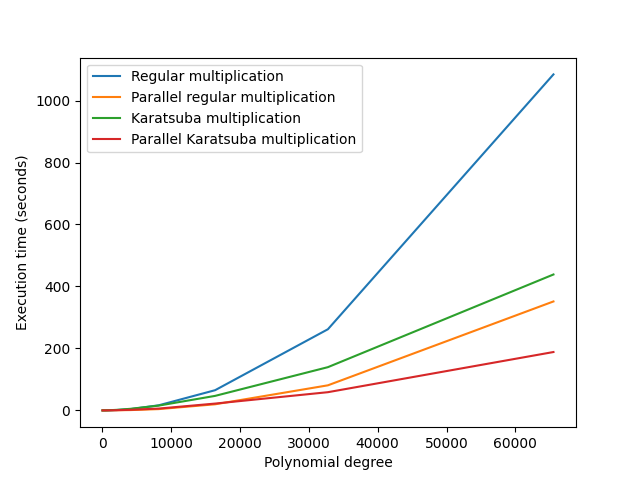
\includegraphics[width=18cm,height=10cm]{execution_time_plot.png}}
		\begin{center} 
		\caption{Line plot containing the polynomial degree on the X-axis and the execution time in seconds on the Y-axis}
		\end{center}
\label{fig}
\end{figure}


\begin{table}[ht]
		\caption{Table with execution times (seconds)} 
\begin{tabular}{c c c c c} 
\hline\hline                        
		Polynomial degree & $ O(n^2) $ seq. & $ O(n^2) $ par. & $ O(n^{\log_2 3}) $ seq. & $ O(n^{\log_2 3}) $ par. \\ [2ex]
\hline\hline                        
		31 & 0.00012 & 0.00137 & 0.00221 & 0.00267 \\    
		63 & 0.00046 & 0.00169 & 0.00746 & 0.00546  \\
		127 & 0.00242 & 0.00259 & 0.02091 & 0.02643  \\
		255  & 0.01338 & 0.00154 & 0.06089 & 0.02689 \\
		511 & 0.05748 & 0.00176 & 0.18336 & 0.07137 \\        
		1023 & 0.24838 & 0.5049 & 0.57698 & 0.21373 \\       
		2047 & 1.01859 & 0.5021 & 1.70614 & 0.69265 \\       
		4095 & 4.06426 & 1.0635 & 5.12932 & 1.94257 \\       
		8191 & 16.4522 & 4.1569 & 15.497 & 5.88652 \\       
		16383 & 65.1912 & 19.7005 & 46.8556 & 22.0241 \\      
		32767 & 261.86 & 80.9225 & 139.531 & 58.7718 \\      
		65535 & 1064.32 & 351.596 & 438.625 & 188.38 \\      
\hline\hline                        
\end{tabular}
\end{table}
	

		
\vspace{12pt}

\end{document}

